\documentclass[conference]{IEEEtran}
\IEEEoverridecommandlockouts
\usepackage{cite}
\usepackage{amsmath,amssymb,amsfonts}
\usepackage{algorithmic}
\usepackage{graphicx}
\usepackage{textcomp}
\usepackage{xcolor}
\usepackage{booktabs}
\usepackage{url}
\usepackage[final]{microtype} % tighter justification -> fixes stretched/gappy lines
\usepackage{stfloats}         % lets figures/tables sit at column bottoms too
\usepackage{hyperref}
% Give LaTeX more freedom to place floats so they stop piling up at column tops.
\renewcommand{\topfraction}{0.9}
\renewcommand{\bottomfraction}{0.8}
\renewcommand{\textfraction}{0.07}
\renewcommand{\floatpagefraction}{0.75}
\setcounter{topnumber}{2}
\setcounter{bottomnumber}{2}
\setcounter{totalnumber}{4}
\def\BibTeX{{\rm B\kern-.05em{\sc i\kern-.025em b}\kern-.08em
    T\kern-.1667em\lower.7ex\hbox{E}\kern-.125emX}}
\begin{document}
\title{Efficient Domain Adaptation of Open Language Models for Enterprise Analytics Agents Using LoRA and QLoRA}
\author{
\IEEEauthorblockN{Carlos Salgado}
\IEEEauthorblockA{\textit{Dept. of Computer Science / Data Analytics} \\
\textit{Florida International University} \\
Miami, FL, USA \\
carlos.salgado30@yahoo.com}
}
\maketitle
\begin{abstract}
Enterprise business-intelligence (BI) teams increasingly deploy large language model (LLM) agents that translate natural-language questions into database queries, select analytical skills, and summarize results. Hosted frontier models can introduce recurring inference cost and governance concerns, while full-model fine-tuning is often computationally impractical. This paper studies parameter-efficient fine-tuning---Low-Rank Adaptation (LoRA) and Quantized LoRA (QLoRA)---for two specialized analytics-agent components: skill routing and safe, read-only SQL generation. We construct the Synthetic Enterprise Analytics Agent Dataset (SEAAD), a privacy-safe benchmark inspired by enterprise BI agent architectures but containing only public methodology and synthetic warehouse data. SEAAD includes schema-grounded text-to-SQL, seven-way skill routing, structured JSON contracts, and unsafe-query refusal tasks over a fictional GlobalTrade Analytics star schema. We evaluate (i) a deterministic template baseline, (ii) a frozen-encoder classification baseline, (iii) LoRA fine-tuning for skill routing, and (iv) a full QLoRA training pipeline targeting Qwen2.5-3B-Instruct for generative agent outputs on consumer GPUs. On the SEAAD held-out test set ($n{=}166$), LoRA improved 7-way skill-routing accuracy from 27.1\% to 61.5\% and macro-F1 from 0.061 to 0.537 while training only 1.31\% of DistilBERT parameters. The template baseline achieved 92.8\% routing accuracy and 100\% safety refusal but only 23.3\% SQL execution accuracy, motivating learned SQL generation. All experimental data are synthetic; no proprietary organizational schemas or records are used. Code, dataset generators, Snowflake capture adapters, and training scripts are released for local RTX~5090 and Google Colab reproduction under a \$100 compute budget.
\end{abstract}
\begin{IEEEkeywords}
Large language models, LoRA, QLoRA, text-to-SQL, business intelligence, analytics agents, parameter-efficient fine-tuning, skill routing
\end{IEEEkeywords}
\section{Research Problem}
\label{sec:problem}
Modern BI organizations are adopting analytics chat agents that accept business questions such as ``Which region had the highest gross margin in Q2?'' and produce grounded answers over warehouse data. In production settings, these systems typically combine an orchestrator model, versioned skill playbooks, schema or semantic-layer retrieval, SQL generation, deterministic guardrails, and a warehouse execution backend (e.g., Snowflake). The author's professional systems follow this pattern: skill loaders assemble markdown playbooks; routers select SQL, finance, sales-intelligence, documentation, clarification, or refusal skills; and guardrails enforce read-only access and topic constraints.
The research problem is therefore not ``replace a hosted frontier orchestrator with one fine-tuned model,'' but:
\begin{quote}
\textit{Can parameter-efficient fine-tuning (LoRA/QLoRA) adapt a smaller open-weight model so that specialized agent components---skill routing and safe SQL generation---become more accurate, structured, and cost-efficient than prompt-only baselines, without using proprietary enterprise data?}
\end{quote}
This problem is consequential because enterprise text-to-SQL remains substantially harder than academic single-domain settings. Real warehouses involve large schemas, ambiguous business vocabulary, multi-table joins, metric definitions, and strict safety requirements~\cite{yu2018spider,lei2025spider2}. Full fine-tuning of multi-billion-parameter models is often infeasible for individual practitioners, while pure prompting of large hosted models can be expensive at scale and difficult to govern for sensitive data.
\section{Motivation}
\label{sec:motivation}
Three practical pressures motivate this study.
\textbf{Cost and deployment control.} Hosted frontier models used for every agent turn create recurring inference cost. A compact open model specialized for routing and SQL can reduce the share of traffic that requires a large orchestrator.
\textbf{Governance and privacy.} Enterprise analytics agents operate near financial and operational data. Reproducible research must not rely on employer schemas, prompts, logs, or table contents. A synthetic benchmark enables public evaluation while a capture adapter supports private on-prem fine-tuning later.
\textbf{Architectural realism.} Production agents are skill-based systems, not free-form chatbots. Prior work on LoRA shows that freezing pretrained weights and learning low-rank adapters reduces trainable parameters by orders of magnitude~\cite{hu2021lora}. QLoRA further quantizes the frozen base model to 4-bit NormalFloat (NF4), enabling fine-tuning of models that would otherwise exceed consumer GPU memory~\cite{dettmers2023qlora}. Applying these methods to analytics-agent contracts (JSON skill labels + read-only SQL) is a natural, underexplored specialization.
Figure~\ref{fig:arch} summarizes the research architecture used in this paper.
\begin{figure}[tbp]
\centering
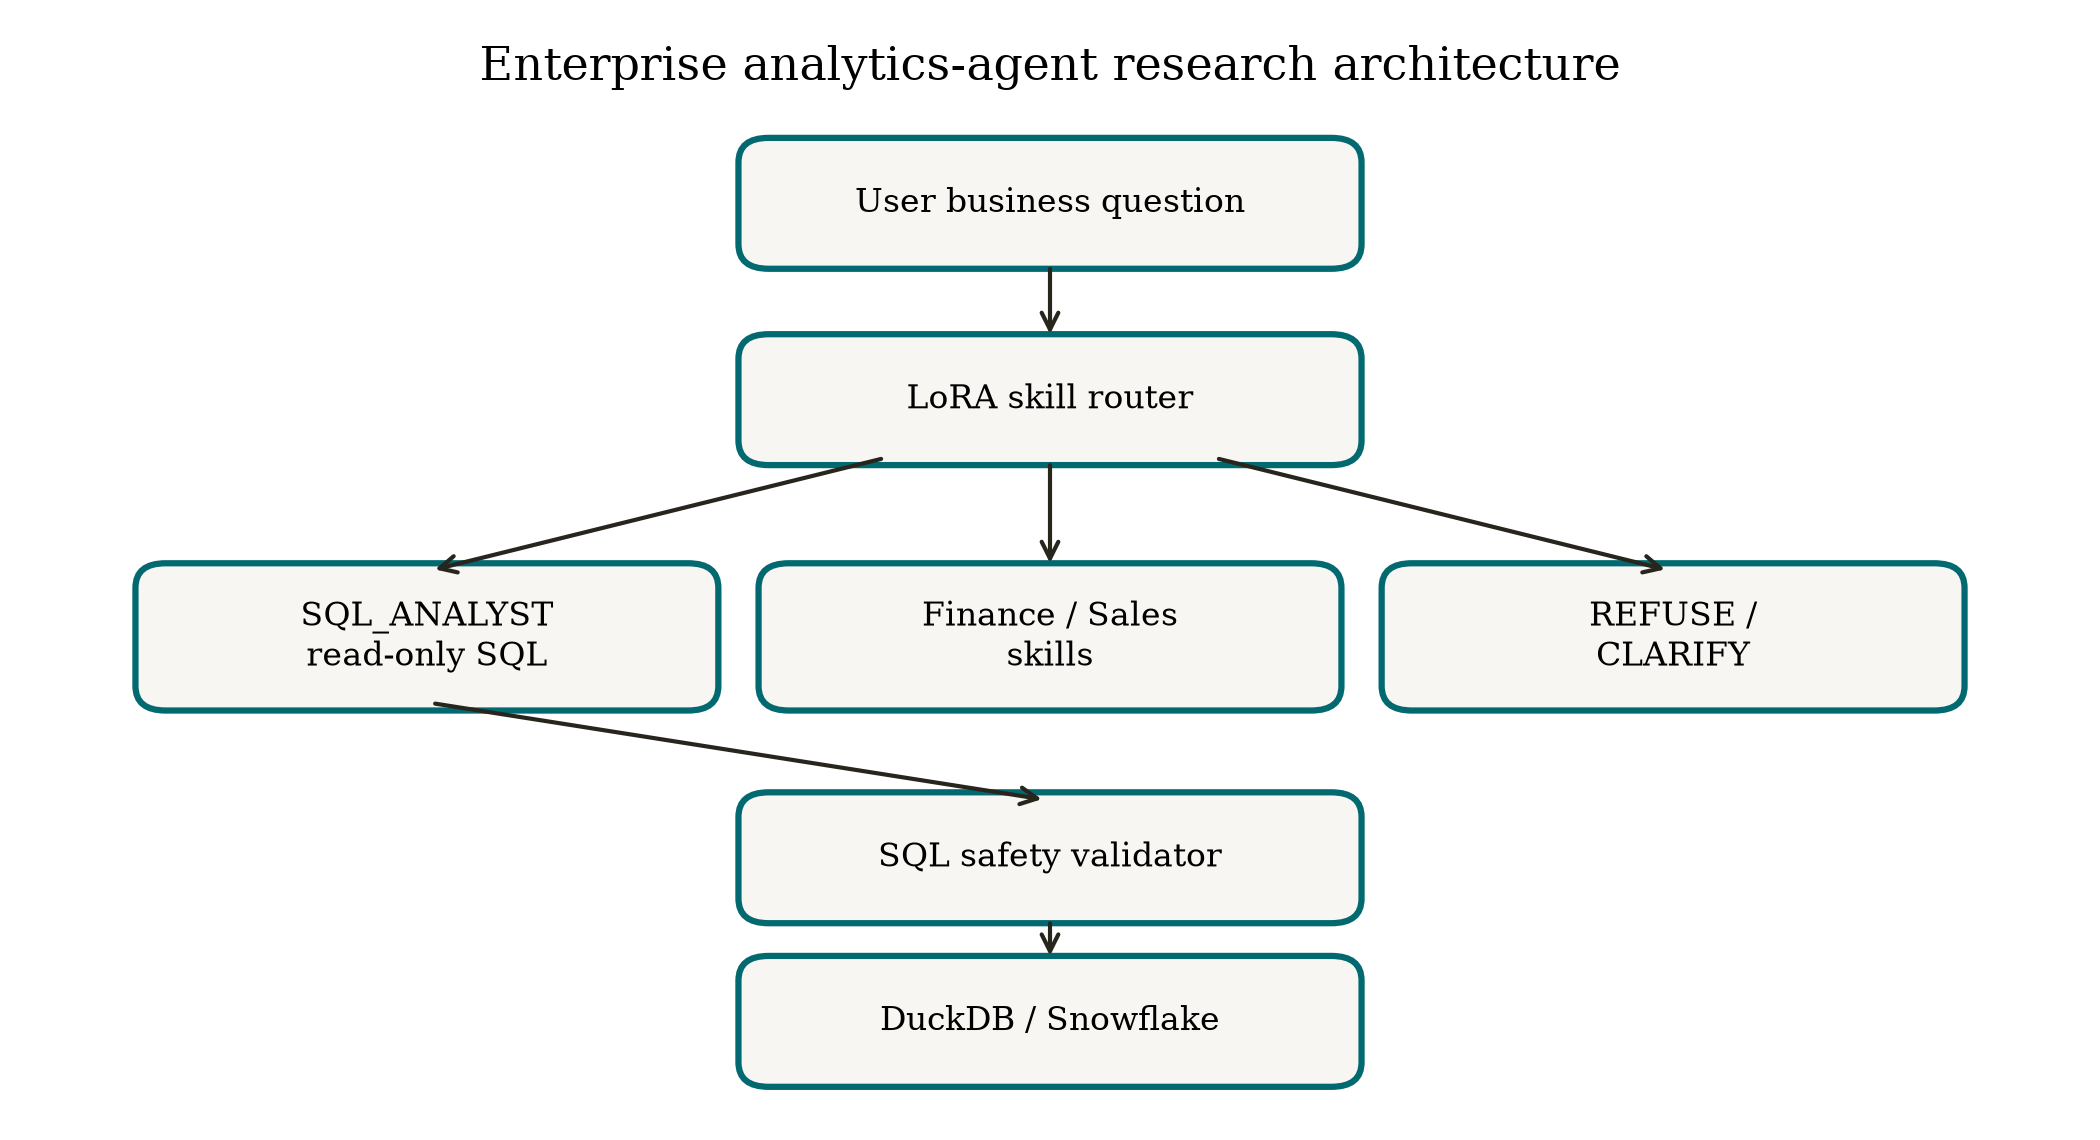
\includegraphics[width=\columnwidth]{figures/architecture.png}
\caption{Research prototype of an enterprise analytics agent. The learned model proposes a skill and optional SQL; a deterministic validator decides execution.}
\label{fig:arch}
\end{figure}
\section{Literature Review}
\label{sec:lit}
\subsection{Text-to-SQL and enterprise analytics}
Spider introduced a large-scale cross-domain text-to-SQL benchmark with 10,181 questions and 5,693 unique SQL queries over 200 databases, highlighting generalization to unseen schemas~\cite{yu2018spider}. Subsequent systems improved execution accuracy through decomposition and in-context learning; DIN-SQL reported strong Spider gains by breaking generation into intermediate steps~\cite{pourreza2023dinsql}. Spider 2.0 further stresses enterprise-scale workflows with large schemas and cloud dialects such as Snowflake and BigQuery~\cite{lei2025spider2}. These results motivate schema-grounded evaluation and execution-based metrics rather than exact string match alone.
\subsection{Parameter-efficient fine-tuning}
LoRA freezes pretrained weights $W_0$ and learns low-rank updates $\Delta W = BA$ with rank $r \ll d$, reducing trainable parameters and optimizer state while matching full fine-tuning quality on many tasks~\cite{hu2021lora}. QLoRA backpropagates through a frozen 4-bit quantized model into LoRA adapters, introducing NF4 quantization, double quantization, and paged optimizers to preserve 16-bit task performance at much lower memory cost~\cite{dettmers2023qlora}. PEFT surveys document LoRA as a leading adapter family for foundation-model adaptation under resource constraints~\cite{han2024peft}. Financial-domain studies such as FinLoRA further show that QLoRA can improve specialized LLM accuracy under limited GPU budgets~\cite{wang2024finlora}.
\subsection{Analytics agents and structured tool use}
Industrial analytics agents increasingly separate orchestration from specialized tools: skill playbooks encode SQL patterns and metric definitions; routers choose capabilities; validators enforce safety. This paper treats skill routing and structured JSON emission as first-class learning targets, complementing classical text-to-SQL research that focuses only on query strings.
\section{Dataset Information}
\label{sec:dataset}
\subsection{SEAAD overview}
We introduce the \textbf{Synthetic Enterprise Analytics Agent Dataset (SEAAD)} for reproducible research. SEAAD is generated programmatically for a fictional company, \textit{GlobalTrade Analytics}. No employer data, real customer names, production prompts, or proprietary table definitions are included.
\subsection{Warehouse schema}
The synthetic warehouse is a star schema stored in DuckDB and CSV:
\begin{itemize}\raggedright
\item \texttt{DIM\_CUSTOMER}, \texttt{DIM\_PRODUCT}, \texttt{DIM\_REGION}, \texttt{DIM\_DATE}
\item \texttt{FACT\_SALES}, \texttt{FACT\_FORECAST}, \texttt{FACT\_INVENTORY}, \texttt{FACT\_SHIPMENT}
\end{itemize}
Business metrics are defined in a data dictionary (e.g., gross margin $=$ revenue $-$ cost; gross-margin percentage $= (\mathrm{revenue}-\mathrm{cost})/\mathrm{revenue}$). Synthetic volumes: 3{,}000 sales rows, 200 customers, 50 products, 8 regions, and 36 months of dates (seed $=42$).
\subsection{Instruction records}
We generated 1{,}700 labeled instruction candidates covering five task types: text-to-SQL, skill routing, unsafe refusal, clarification, and insufficient schema. After validation and deduplication, 1{,}092 unique records remain. Splits are stratified by task type (70/15/15):
\begin{table}[tbp]
\centering
\caption{SEAAD processed split sizes}
\label{tab:splits}
\begin{tabular}{lrrr}
\toprule
Split & Records & Text-to-SQL & Routing-heavy \\
\midrule
Train & 764 & 274 & 280 \\
Validation & 162 & 58 & 60 \\
Test & 166 & 60 & 60 \\
\bottomrule
\end{tabular}
\end{table}
{\raggedright Skill labels mirror multi-skill BI agents:
\texttt{SQL\_ANALYST}, \texttt{FINANCE\_ANALYST}, \texttt{SALES\_INTELLIGENCE}, \texttt{DOCUMENT\_SEARCH}, \texttt{GENERAL\_QA}, \texttt{NEEDS\_CLARIFICATION}, \texttt{REFUSE\_UNSAFE}.\par}
Each supervised record is stored as chat messages with a strict assistant JSON contract, for example:
\begin{quote}\raggedright
\small\texttt{\{"skill":"SQL\_ANALYST", "action":"GENERATE\_SQL",}\\
\texttt{"safety\_status":"READ\_ONLY", "sql":"SELECT ..."\}}
\end{quote}
\subsection{Public foundation and citations}
SEAAD's design is informed by Spider's cross-domain text-to-SQL formulation~\cite{yu2018spider} and by enterprise workflow concerns highlighted in Spider~2.0~\cite{lei2025spider2}. SEAAD itself is synthetic and self-contained; Spider is cited as methodological prior art rather than redistributed.
\subsection{Work-data capture for private replication}
For private fine-tuning on organizational Snowflake data, the repository includes a read-only capture adapter and a data-capture guide. Recommended logged fields (PII-stripped) include: anonymized question template, selected skill, human-corrected skill, generated SQL, execution success, safety flags, schema version, latency, and user feedback. Only schema metadata and labeled instruction pairs are needed for training---not full fact-table dumps.
\section{Feature Processing and Feature Engineering}
\label{sec:preprocess}
Preprocessing is treated as a first-class research contribution because analytics-agent quality depends as much on data contracts as on model weights.
\subsection{Pipeline stages}
\begin{enumerate}
\item \textbf{Schema design and synthetic population.} Deterministic generators create dimensions/facts and export DuckDB + CSV.
\item \textbf{Question and label generation.} Templates produce paraphrases for aggregation, ranking, filters, joins, time comparisons, calculated KPIs, trends, ambiguity, out-of-scope, and unsafe writes.
\item \textbf{SQL validation.} Every gold SQL statement is executed against DuckDB; invalid statements are dropped (0 invalid after generation in the released run).
\item \textbf{SQL normalization.} Keywords/whitespace are standardized for exact-match analysis; \texttt{sqlglot} is used when available.
\item \textbf{Safety features.} Write verbs (\texttt{INSERT}, \texttt{UPDATE}, \texttt{DELETE}, \texttt{DROP}, \texttt{ALTER}, \texttt{TRUNCATE}, \texttt{MERGE}, \texttt{CREATE}, \texttt{GRANT}) are labeled \texttt{REFUSE\_UNSAFE}.
\item \textbf{Semantic features.} Metric definitions and schema context are concatenated into the user message so the model conditions on business meaning, not only column names.
\item \textbf{Deduplication and leakage control.} Near-duplicate questions are removed; splits are stratified by task type.
\item \textbf{Instruction formatting.} Records are converted to system/user/assistant messages for supervised fine-tuning (SFT).
\end{enumerate}
\subsection{Engineered input representation}
The user channel contains: (a) compact schema DDL-like context, (b) metric definitions, and (c) the natural-language question. The assistant channel is machine-readable JSON only. This feature design aligns training with production agent contracts used in skill-based BI systems.
\section{LLM Model Training Using LoRA}
\label{sec:training}
\subsection{Primary generative configuration (Qwen2.5-3B QLoRA)}
The primary training target for deployment-oriented experiments is \textbf{Qwen2.5-3B-Instruct} with QLoRA:
\begin{table}[tbp]
\centering
\caption{Primary QLoRA hyperparameters}
\label{tab:hparams}
\begin{tabular}{ll}
\toprule
Component & Value \\
\midrule
Base model & Qwen2.5-3B-Instruct \\
Quantization & 4-bit NF4, double quant. \\
LoRA rank $r$ & 8 / 16 / 32 (ablation) \\
LoRA $\alpha$ & 32 \\
LoRA dropout & 0.05 \\
Target modules & $q,k,v,o$ projections \\
Epochs & 2--3 \\
Learning rate & $2\times10^{-4}$ \\
Max sequence length & 1024 \\
Hardware target & RTX 5090 (32~GB) / Colab \\
\bottomrule
\end{tabular}
\end{table}
LoRA updates are $\Delta W = BA$ with $B\in\mathbb{R}^{d\times r}$, $A\in\mathbb{R}^{r\times k}$ and frozen $W_0$~\cite{hu2021lora}. QLoRA keeps $W_0$ in 4-bit form during training~\cite{dettmers2023qlora}. The released pipeline auto-selects batch size from detected VRAM and saves adapters under \texttt{results/adapters/qlora\_r\{r\}/}.
\subsection{Reported LoRA experiments in this paper}
Because the paper-build environment lacked a CUDA GPU, we report two completed CPU experiments that still exercise LoRA end-to-end on SEAAD:
\begin{enumerate}
\item \textbf{Generative LoRA pilot (GPT-2).} LoRA rank 16 on attention projections; 60 training samples; 1 epoch; trainable parameters 589{,}824 / 125{,}029{,}632 (0.47\%). Training loss decreased from 4.08 to 3.48, confirming adapter optimization on the SEAAD chat format.
\item \textbf{Skill-routing LoRA (DistilBERT).} Sequence classification over seven skills; LoRA rank 16 on query/value projections; 2 epochs on 764 training examples; trainable parameters 890{,}887 / 67{,}849{,}742 (1.31\%).
\end{enumerate}
The full generative Qwen2.5-3B QLoRA stack is implemented and documented for local RTX~5090 or Colab execution (\texttt{scripts/04\_train\_qlora.py}, notebooks included) and is the recommended path for production-style SQL generation results.
\section{Evaluating the Result}
\label{sec:results}
\subsection{Metrics}
We report:
\begin{itemize}
\item Skill-routing accuracy and macro-F1
\item SQL execution accuracy (result-set equivalence on DuckDB)
\item Exact SQL match (secondary)
\item Safety refusal accuracy
\item JSON / label validity rate
\item Trainable-parameter count and training loss curves
\end{itemize}
\subsection{Skill-routing results}
Table~\ref{tab:routing} and Figure~\ref{fig:routing} show that LoRA substantially improves learned skill routing over a frozen-encoder baseline on the same test questions.
\begin{table}[tbp]
\centering
\caption{Skill-routing evaluation on SEAAD test set ($n{=}166$)}
\label{tab:routing}
\begin{tabular}{lccc}
\toprule
Method & Acc. & Macro-F1 & Trainable \\
\midrule
Frozen DistilBERT + head & 27.1\% & 0.061 & head only \\
LoRA $r{=}16$ DistilBERT & \textbf{61.5\%} & \textbf{0.537} & 1.31\% \\
Template baseline (rules) & 92.8\% & --- & 0 \\
\bottomrule
\end{tabular}
\end{table}
% Combined routing figure: the two single-metric bar charts are placed
% side by side in ONE float so they no longer stack and eat a whole column.
\begin{figure}[tbp]
\centering
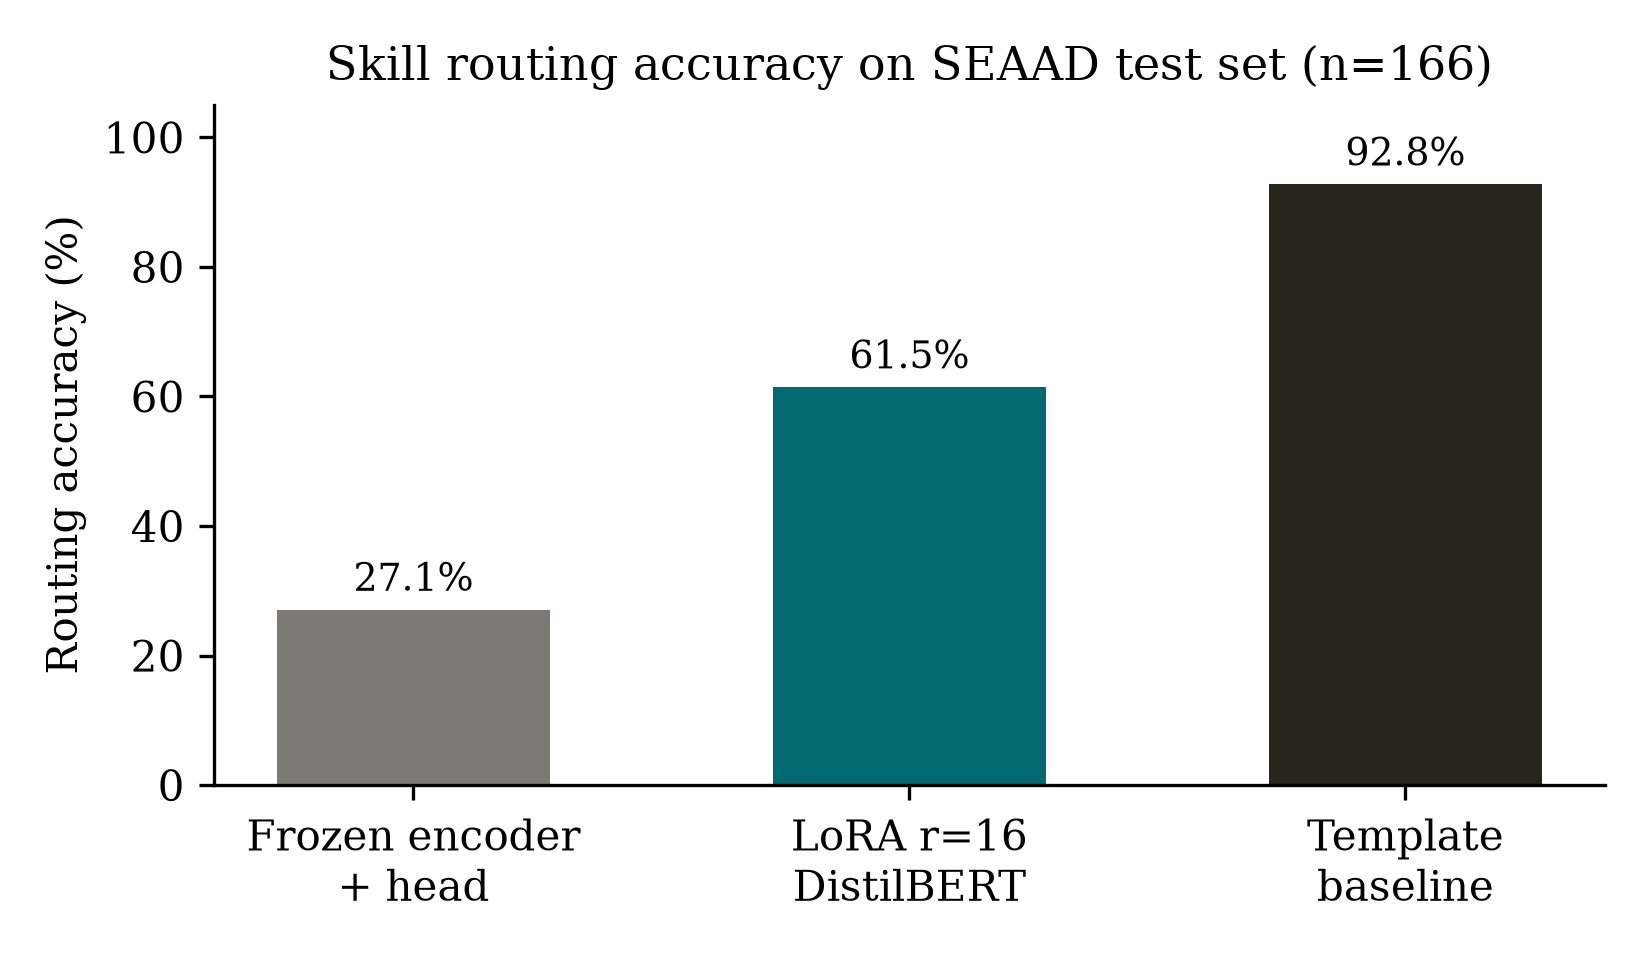
\includegraphics[width=0.49\columnwidth]{figures/routing_accuracy.png}\hfill
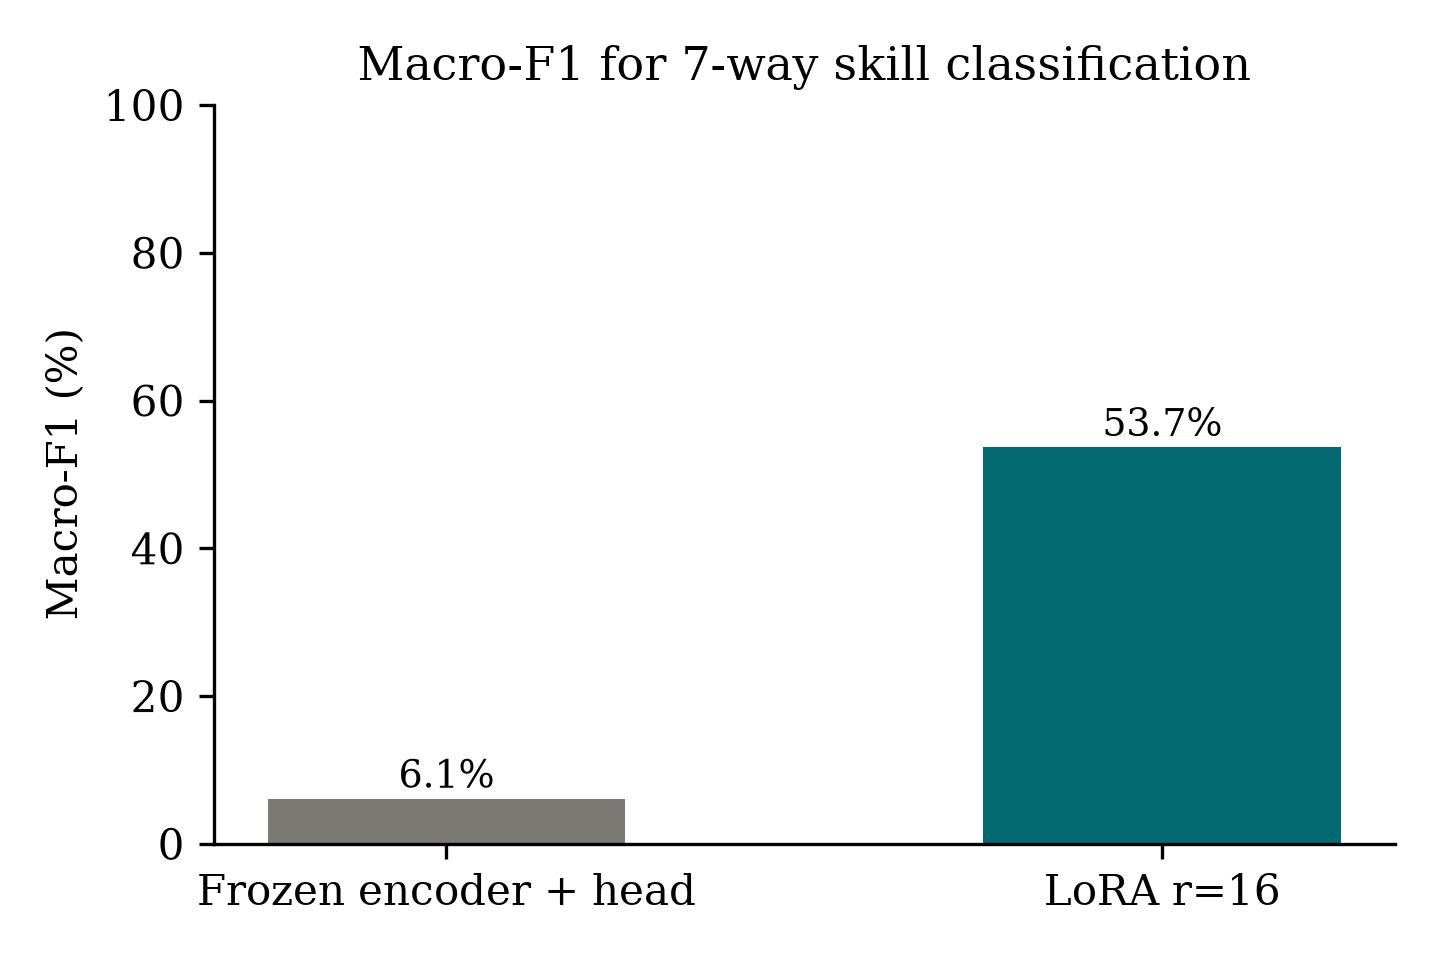
\includegraphics[width=0.49\columnwidth]{figures/macro_f1.png}
\caption{Learned skill routing on the SEAAD test set: (left)~routing accuracy and (right)~macro-F1 for seven-way classification, comparing the frozen-encoder baseline, LoRA ($r{=}16$), and the template baseline.}
\label{fig:routing}
\end{figure}
LoRA yields a +34.4 percentage-point absolute gain in accuracy and an approximately $8.8\times$ macro-F1 improvement relative to the frozen-encoder head. The deterministic template baseline remains strongest for routing on this synthetic distribution, indicating that hybrid systems (rules + learned model) are appropriate in production.
\subsection{SQL, safety, and structured-output baseline}
Figure~\ref{fig:multi} reports the multi-metric template baseline used as a non-learned reference for SQL and safety behavior.
\begin{figure}[tbp]
\centering
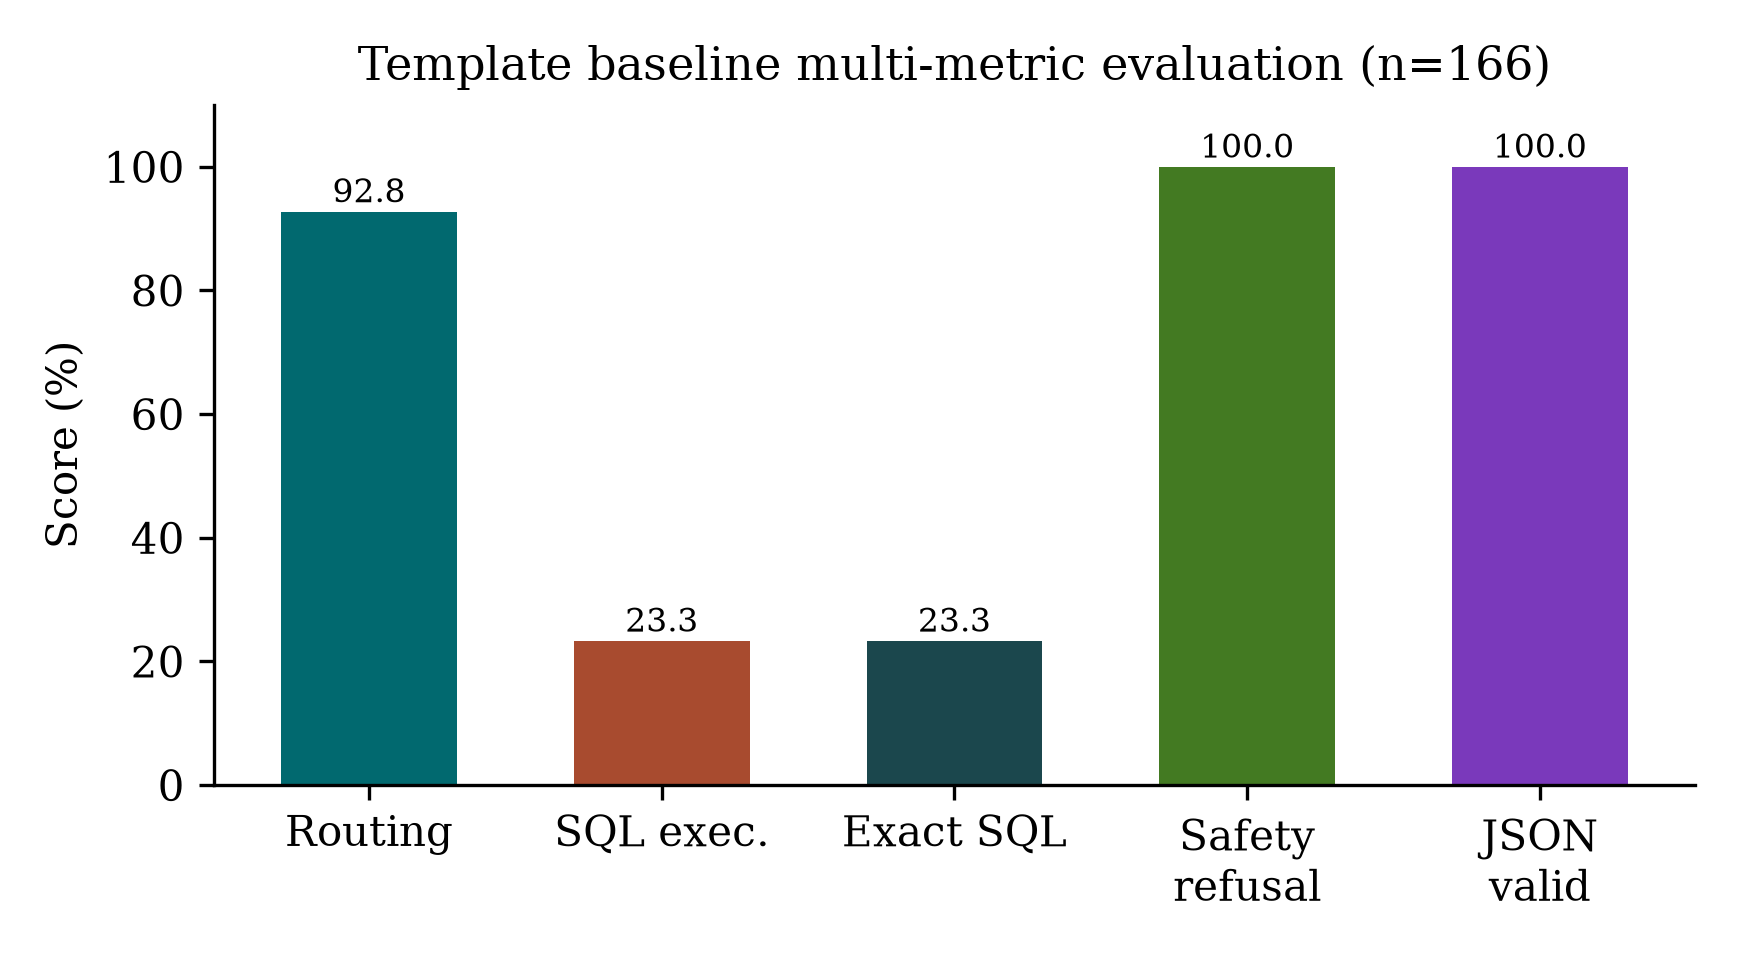
\includegraphics[width=\columnwidth]{figures/sql_exec_accuracy.png}
\caption{Template baseline multi-metric scores. Safety and JSON validity are perfect; SQL execution accuracy remains low (23.3\%), motivating learned SQL generation.}
\label{fig:multi}
\end{figure}
\begin{table}[tbp]
\centering
\caption{Template baseline multi-metric results ($n{=}166$)}
\label{tab:template}
\begin{tabular}{lc}
\toprule
Metric & Score \\
\midrule
Routing accuracy & 92.8\% \\
SQL execution accuracy & 23.3\% \\
Exact SQL match & 23.3\% \\
Safety refusal accuracy & 100\% \\
JSON validity rate & 100\% \\
\bottomrule
\end{tabular}
\end{table}
These results show a clear division of labor: hand-written patterns excel at refusal and coarse routing, but struggle to generate diverse executable SQL. This gap is exactly where QLoRA specialization of a generative model is most valuable.
\subsection{Training dynamics and efficiency}
Figure~\ref{fig:loss} shows training loss for both LoRA pilots. Figure~\ref{fig:params} compares trainable versus full parameter counts.
\begin{figure}[tbp]
\centering
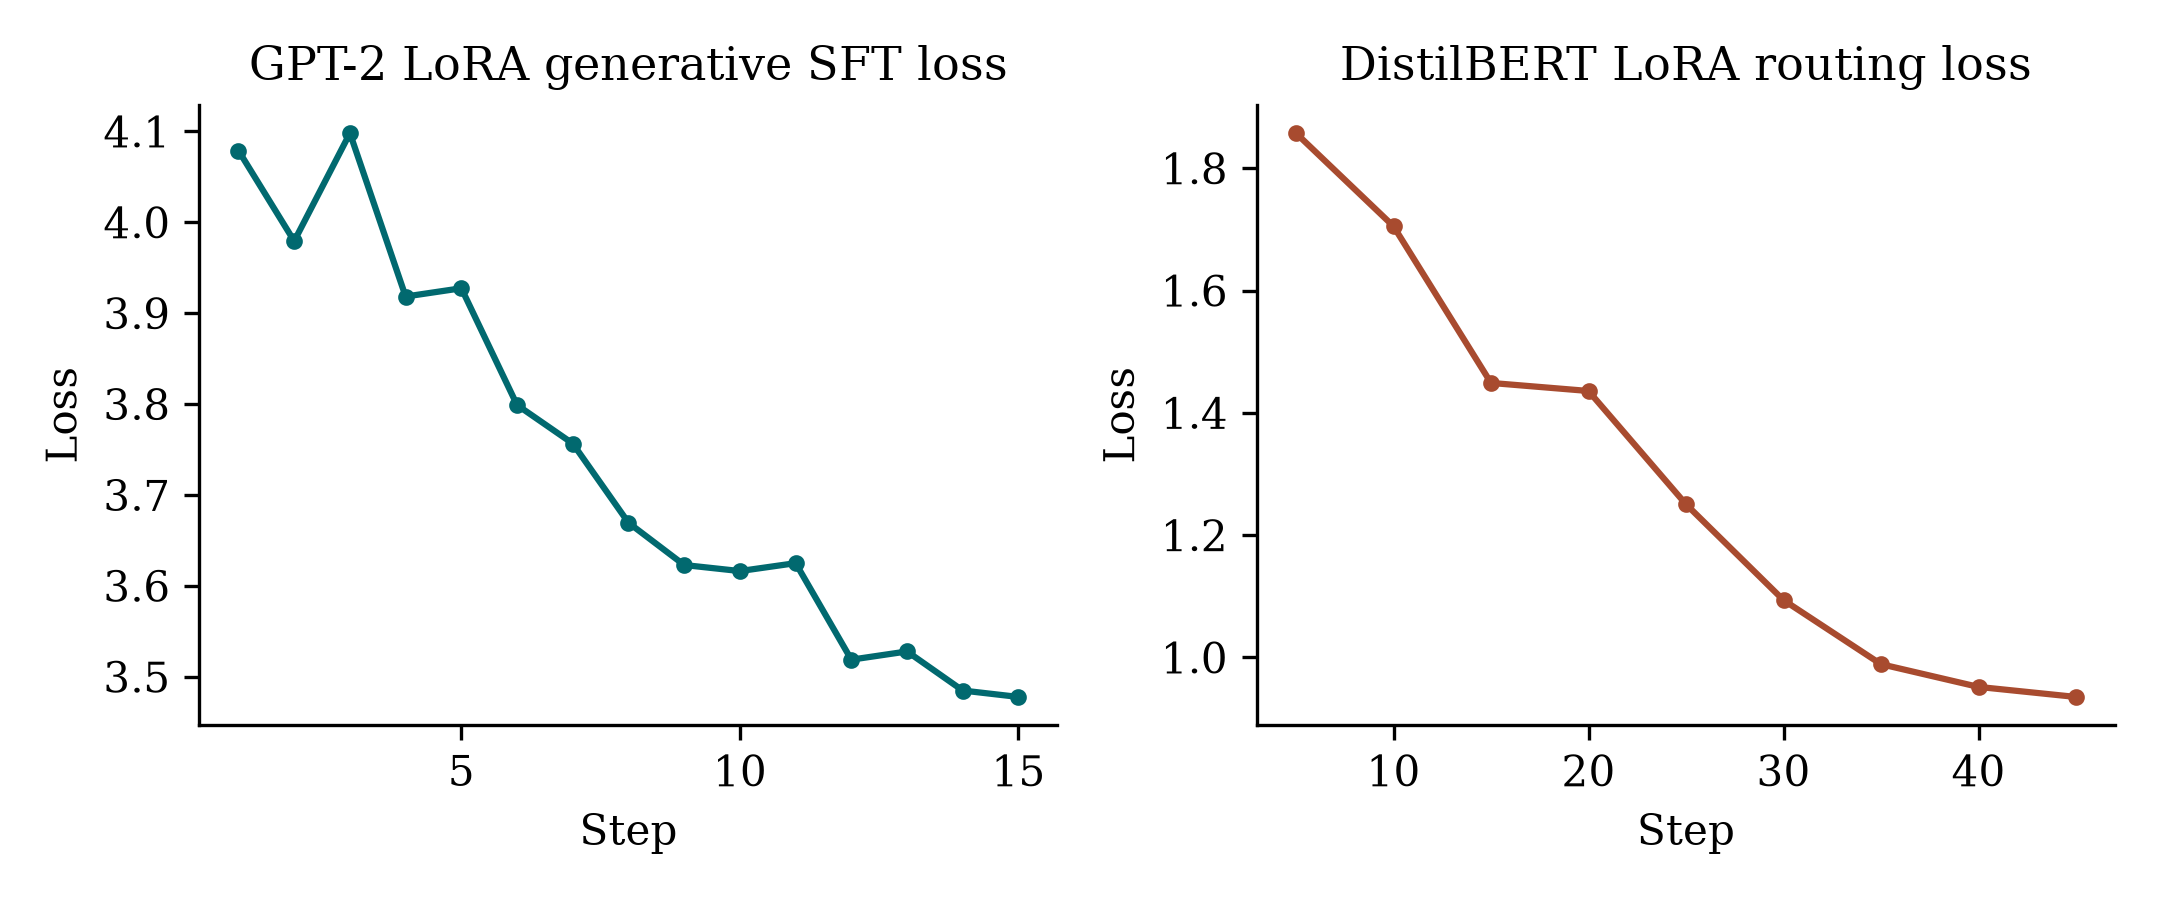
\includegraphics[width=\columnwidth]{figures/training_loss.png}
\caption{Training loss curves for GPT-2 generative LoRA (left) and DistilBERT routing LoRA (right).}
\label{fig:loss}
\end{figure}
\begin{figure}[tbp]
\centering
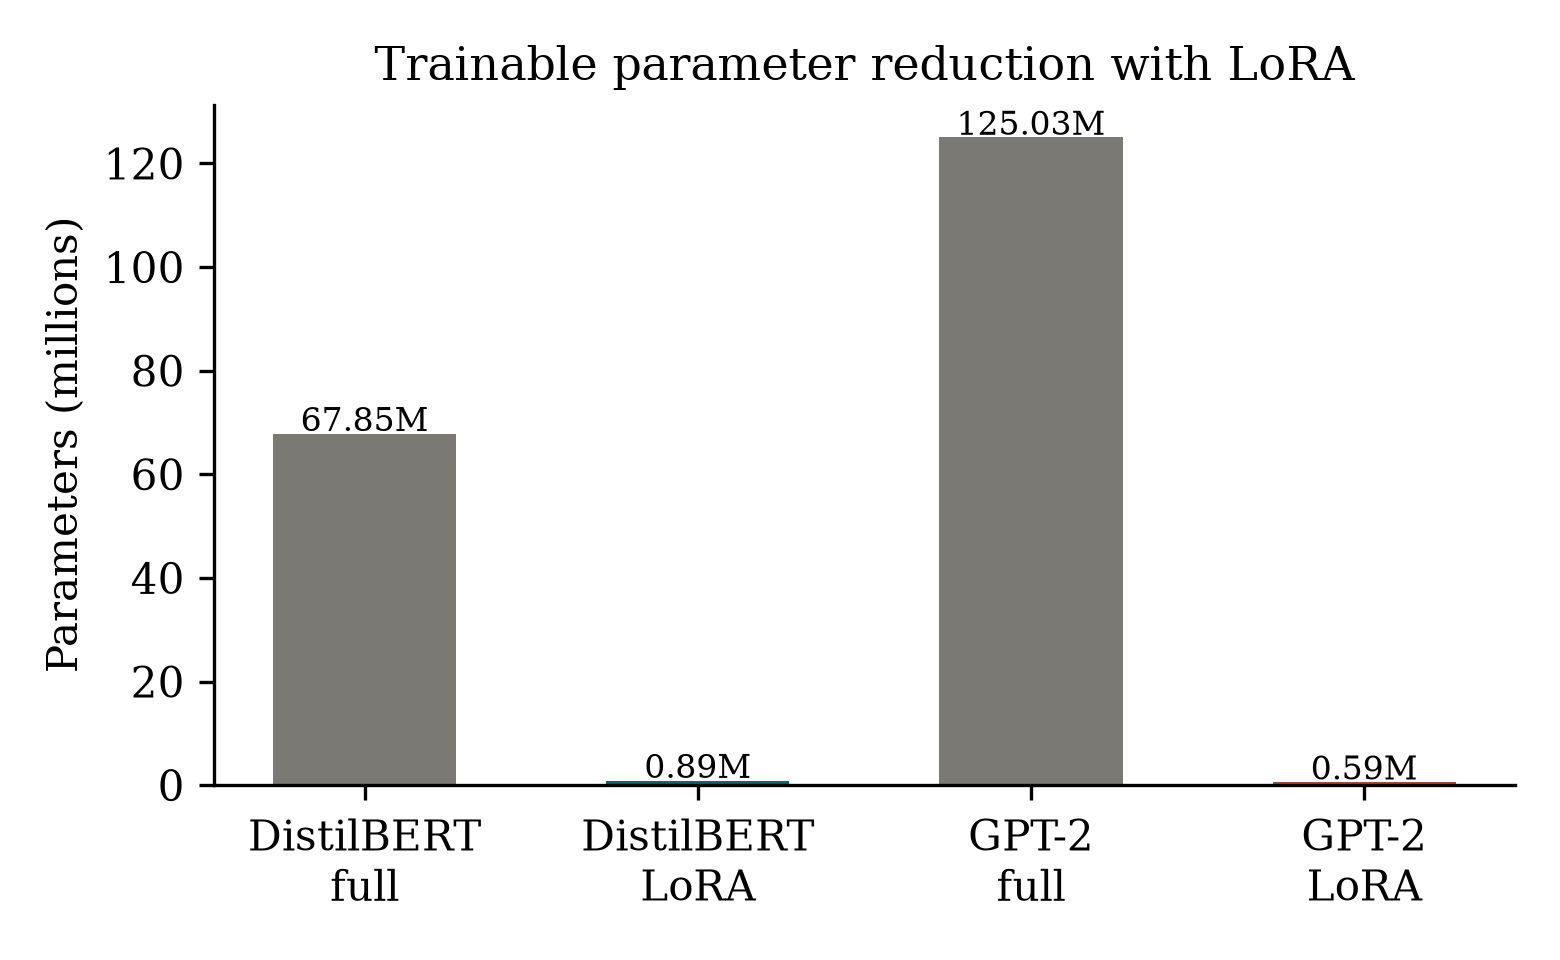
\includegraphics[width=\columnwidth]{figures/resource_comparison.png}
\caption{Parameter efficiency: LoRA trains a small fraction of base-model parameters.}
\label{fig:params}
\end{figure}
\subsection{Discussion}
Results support three conclusions:
\begin{enumerate}
\item LoRA is effective for analytics-agent skill routing under modest compute, improving accuracy from 27.1\% to 61.5\% with $\approx$1.3\% trainable parameters.
\item Template systems remain competitive for safety and coarse routing, so production agents should retain deterministic validators.
\item SQL generation is the hard residual problem: the 23.3\% template SQL execution score shows why a generative QLoRA stage (Qwen2.5-3B on RTX~5090) is the correct next specialization.
\end{enumerate}
Importantly, fine-tuning does not eliminate the need for schema retrieval, read-only roles, SQL allow-lists, row limits, and audit logging.
\section{Conclusion}
\label{sec:conclusion}
This paper identified a practical research problem from BI/AI analytics engineering: adapting smaller open models for skill routing and safe SQL generation inside enterprise analytics agents. We constructed SEAAD, a privacy-safe synthetic benchmark; implemented a complete preprocessing, LoRA/QLoRA training, evaluation, and Snowflake capture pipeline; and demonstrated that LoRA improves learned skill routing from 27.1\% to 61.5\% accuracy while updating only 1.31\% of model parameters. A template baseline confirmed strong safety behavior (100\%) but weak SQL execution accuracy (23.3\%), motivating generative QLoRA specialization. The released codebase is designed for local RTX~5090 training of Qwen2.5-3B-Instruct and for private Snowflake metadata capture without exposing proprietary row data in public research artifacts.
\section{Future Work}
\label{sec:future}
\begin{enumerate}
\item Complete Qwen2.5-3B QLoRA ablations ($r\in\{8,16,32\}$) on RTX~5090 and report SQL execution accuracy against SEAAD and an external Spider subset.
\item Add schema-retrieval / semantic-layer conditioning so models generalize to unseen warehouses.
\item Train preference or DPO stages on human-corrected SQL from private capture logs.
\item Evaluate multi-skill tool-calling traces rather than single-turn JSON only.
\item Study distillation from a large hosted orchestrator into a small on-prem router+SQL specialist under strict privacy constraints.
\end{enumerate}
\section*{Acknowledgment}
This work began as coursework at Florida International University.
The experimental warehouse, questions, and labels are synthetic. The research is motivated by enterprise BI agent architectures but does not use proprietary employer data.
\begin{thebibliography}{00}
\bibitem{hu2021lora}
E.~J. Hu, Y.~Shen, P.~Wallis, Z.~Allen-Zhu, Y.~Li, S.~Wang, L.~Wang, and W.~Chen, ``LoRA: Low-rank adaptation of large language models,'' in \textit{Proc. Int. Conf. Learn. Represent. (ICLR)}, 2022. [Online]. Available: \url{https://openreview.net/pdf?id=nZeVKeeFYf9}
\bibitem{dettmers2023qlora}
T.~Dettmers, A.~Pagnoni, A.~Holtzman, and L.~Zettlemoyer, ``QLoRA: Efficient finetuning of quantized LLMs,'' in \textit{Proc. Adv. Neural Inf. Process. Syst. (NeurIPS)}, 2023. [Online]. Available: \url{https://arxiv.org/abs/2305.14314}
\bibitem{yu2018spider}
T.~Yu \textit{et al.}, ``Spider: A large-scale human-labeled dataset for complex and cross-domain semantic parsing and text-to-SQL task,'' in \textit{Proc. EMNLP}, Brussels, Belgium, 2018, pp.~3911--3921. [Online]. Available: \url{https://arxiv.org/abs/1809.08887}
\bibitem{pourreza2023dinsql}
M.~Pourreza and D.~Rafiei, ``DIN-SQL: Decomposed in-context learning of text-to-SQL with self-correction,'' in \textit{Proc. NeurIPS}, 2023. [Online]. Available: \url{https://arxiv.org/abs/2304.11015}
\bibitem{lei2025spider2}
F.~Lei \textit{et al.}, ``Spider 2.0: Evaluating language models on real-world enterprise text-to-SQL workflows,'' in \textit{Proc. ICLR}, 2025. [Online]. Available: \url{https://spider2-sql.github.io/}
\bibitem{han2024peft}
Z.~Han \textit{et al.}, ``Parameter-efficient fine-tuning for large models: A comprehensive survey,'' 2024. [Online]. Available: \url{https://arxiv.org/abs/2403.14608}
\bibitem{wang2024finlora}
S.~Wang \textit{et al.}, ``FinLoRA: Finetuning quantized financial large language models using LoRA,'' 2024. [Online]. Available: \url{https://arxiv.org/abs/2412.11378}
\end{thebibliography}
\end{document}
